\ifthenelse{\equal{\Langue}{FR}}{
\chapter{Production autonome d'énergie pour site isolé}
}{
\chapter{Autonomous energy production for isolated site}
}

%%%%%%% Introduction %%%%%%%
\ifthenelse{\equal{\Langue}{FR}}{
\textit{Nota: Les dispositifs et dimensionnements présentés ci-après constituent une approche simplifiée du problème.}

Le cadre est celui d'un site isolé, que l'on souhaite alimenter à partir de panneaux photovoltaïques (PV) et batteries de stockage.

Le site consomme de l'énergie en permanence avec une puissance ``talon'' et des pointes de consommations au cours de la journée. 

Pour maintenir un fonctionnement durant la nuit, un stockage d'énergie par batteries est associé aux PV\@.

La fourniture d'énergie est faite en courant alternatif, la tension de service de 230~VAC, 50~Hz étant générée au moyen d'un onduleur monophasé.

L'architecture générale du dispositif est ainsi la suivante:
}{
\textit{Note: The devices and sizing presented below are a simplified approach to the problem.}

The context is that of an isolated site that we want to power using photovoltaic (PV) panels and storage batteries.

The site consumes energy continuously with a ``base'' power and consumption peaks throughout the day.

To maintain operation during the night, energy storage by batteries is associated with the PV panels.

The energy supply is provided in alternating current, with a service voltage of 230~VAC, 50~Hz generated by a single-phase inverter.

The general architecture of the system is as follows:
}

\begin{figure}[ht]
\centering
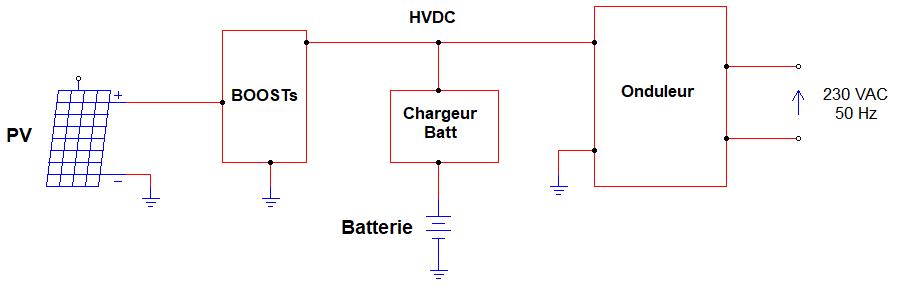
\includegraphics[width=0.8\linewidth]{TD_Boost_2Q_Onduleur/fig/Archi_Globale.png}
\caption{Architecture globale}
\end{figure}

\ifthenelse{\equal{\Langue}{FR}}{
\textbf{Données principales}
}{
\textbf{Main data}
}

\underline{Installation:}
\begin{itemize}
\ifthenelse{\equal{\Langue}{FR}}{
\item Puissance talon de l'installation: 300 W
\item Pointes de puissance consommée: 1500 W
\item Durée des pointes de puissance: 3*30 mn entre 11h00 et 15h00.
\end{itemize}

\underline{PV:}
\begin{itemize}
\item Les PV sont orientés au sud, avec une inclinaison de $35^\circ$. L'installation se trouve dans les Alpes, au sud de Briançon, dans une zone géographique où l'irradiation moyenne annuelle est de $1500\ kWh/m^2$ (en tenant compte des ombrages portés).

\item La data sheet d'un PV donne les informations suivantes:
}{
\item Base power of the installation: 300 W
\item Peak power consumption: 1500 W
\item Duration of power peaks: 3$\times$30 min between 11:00 and 15:00.
\end{itemize}

\underline{PV panels:}
\begin{itemize}
\item The PV panels are oriented to the south, with an inclination of $35^\circ$. The installation is located in the Alps, south of Briançon, in a geographical area where the average annual irradiation is $1500\ kWh/m^2$ (taking into account shading).

\item The datasheet of a PV panel provides the following information:
}

\clearpage
\begin{centering}
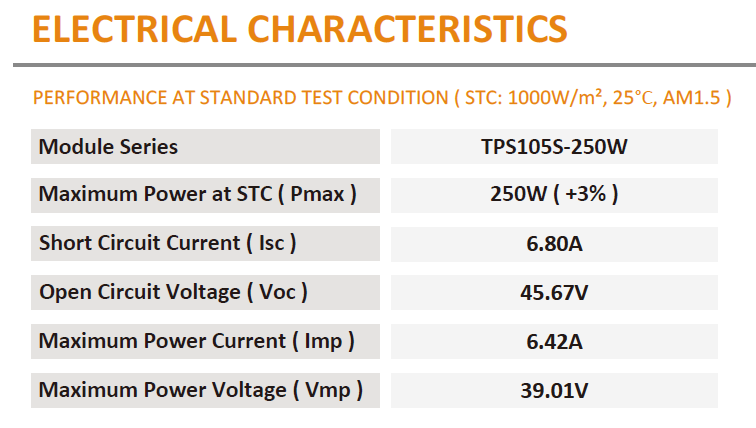
\includegraphics[width=0.49\linewidth]{TD_Boost_2Q_Onduleur/fig/elec_specif.png}
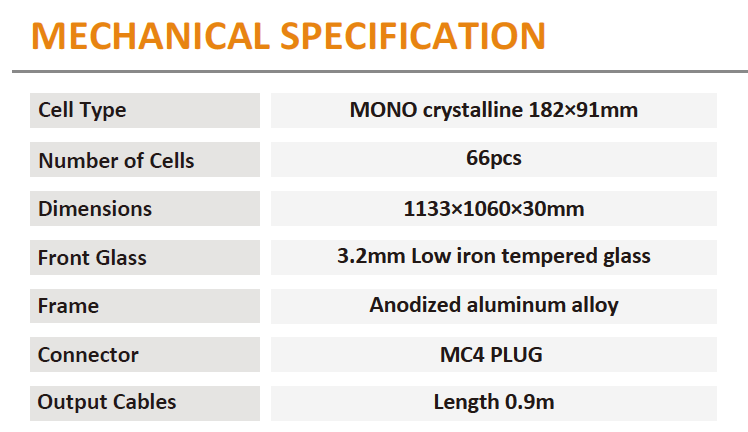
\includegraphics[width=0.49\linewidth]{TD_Boost_2Q_Onduleur/fig/meca_specif.png}
\end{centering}

\ifthenelse{\equal{\Langue}{FR}}{
\item Le rendement global des PV est de 20 \% (tenant compte du ratio\newline [surface cellules / surface totale]) et on considère que le rendement global de la chaîne de conversion d'énergie est de 90 \% (cumul de convertisseurs, pertes en lignes, …).
}{
\item The overall efficiency of the PV panels is 20\% (taking into account the ratio [cell area / total area]) and it is considered that the overall efficiency of the energy conversion chain is 90\% (including converters, line losses, etc.).
}

\end{itemize}

%%%%%% Partie 0 %%%%%%

\ifthenelse{\equal{\Langue}{FR}}{
\section*{Préliminaires}
Déterminer:
}
{
\section*{Preliminaries}
Determine:
}
\begin{enumerate}

\ifthenelse{\equal{\Langue}{FR}}{
\item L'énergie consommée par l'installation par jour et sur une année.
}{
\item The energy consumed by the installation per day and per year.
}

\ifthenelse{\equal{\SuCorr}{CO}}{
$\begin{aligned}
E_{\text{year }}=\overbrace{300 \times 24 \times 365}^{\text{average }}+\overbrace{1500 \times 3 \times 0.5 \times 365}^{\text{peak}} &=  3.45 \text{ MWh/year}\\
&=  9.45 \text{ kWh/day} 
\end{aligned}$
}


\ifthenelse{\equal{\Langue}{FR}}{
\item La surface nécessaire de PV pour permettre l'alimentation du dispositif en tenant compte des rendements.
}{
\item The required PV panel area to supply the system, taking into account the efficiencies.
}

\ifthenelse{\equal{\SuCorr}{CO}}{
\ifthenelse{\equal{\Langue}{FR}}{Avec}{With} $1520 \text{ kWh} / \text{m}^2 / \text{year}$

\vspace{0.25cm}
$\begin{aligned}
& \left.\begin{array}{l}
\eta_{\text{PV}}=20 \% \\
\eta_{\text{Elec}}=90 \%
\end{array}\right\} 18 \% \Rightarrow 270 \text{ kWh} / \mathrm{m}^2 / \text{year (Elec energy)}
\end{aligned}$

\[S=\frac{3.45 \cdot 10^3}{270}=12.8 \text{m}^2\]
}

\ifthenelse{\equal{\Langue}{FR}}{
\item Le nombre minimum de PV nécessaires.
}{
\item The minimum number of PV panels required.
}

\ifthenelse{\equal{\SuCorr}{CO}}{
\ifthenelse{\equal{\Langue}{FR}}{Nombre de panneaux:}{Number of panels:} $\frac{12.8}{1,13 \times 1,06}=10,7 \Rightarrow 11$ \ifthenelse{\equal{\Langue}{FR}}{panneaux}{panels}.\ ($1.13 m^2 = $ \ifthenelse{\equal{\Langue}{FR}}{Surface d'1 panneau}{Surface of 1 panel})
}

\end{enumerate}

%%%%%%% Partie 1 %%%%%%

\ifthenelse{\equal{\Langue}{FR}}{
\section{Convertisseurs BOOST}

On décide d'implanter \textbf{12 PV}, associés en deux groupes de PV en série. Chaque groupe de PV est connecté à une entrée d'un convertisseur DC-DC de type BOOST\@.
Ainsi, la structure développée du ``BOOST'' de la figure 1 est la suivante:
}{
\section{BOOST Converters}

It is decided to implement \textbf{12 PV panels}, grouped in two series-connected PV panel groups. Each PV panel group is connected to an input of a BOOST DC-DC converter.
Thus, the developed structure of the ``BOOST'' in Figure 1 is as follows:
}\label{sec:Convertisseur_BOOST}

\begin{figure}[ht]
\centering
\includegraphics[width=0.6\linewidth]{TD_Boost_2Q_Onduleur/fig/Archi_Boost.png}
\caption{Architecture Boost}
\end{figure}

\ifthenelse{\equal{\Langue}{FR}}{
On suppose que tous les PV sont éclairés de façon uniforme de sorte que chaque groupe de PV fourni la moitié de la puissance instantanée consommée.

La tension de sortie HVDC est asservie à \textbf{500 V} par des boucles de régulation agissant sur les rapports cycliques des transistors Q1 et Q2.

La fréquence de découpage de Q1 et Q2 est fixe et égale à \textbf{Fd = 50 kHz}.

\underline{On ne s'intéresse pour l'instant qu'au BOOST 1 et on suppose que tous les composants}\newline
\underline{sont parfaits.}

En considérant que:
\begin{itemize}
\item la tension d'entrée du BOOST (sur C1) et HVDC sont rigoureusement constantes sur une période de découpage
\item l'ondulation de courant c-à-c $\Delta I$ dans L1 représentent 20 \% du courant moyen d'entrée.
\item On se place dans un régime de conduction continue.
\end{itemize}
}{
It is assumed that all PV panels are uniformly illuminated so that each PV panel group provides half of the instantaneous power consumed.

The HVDC output voltage is regulated at \textbf{500 V} by control loops acting on the duty cycles of transistors Q1 and Q2.

The switching frequency of Q1 and Q2 is fixed and equal to \textbf{Fd = 50 kHz}.

\underline{For now, we are only interested in BOOST 1 and we assume that all components are ideal.}

Considering that:
\begin{itemize}
\item The BOOST input voltage (on C1) and HVDC are rigorously constant over one switching period.
\item The ripple current $\Delta I$ in L1 represents 20\% of the average input current.
\item We are in continuous conduction mode.
\end{itemize}
}


\begin{enumerate}
\ifthenelse{\equal{\Langue}{FR}}{
\item Représenter les courants dans L1, Q1 et D1 ainsi que les tensions à leurs bornes, sur deux périodes de découpage et pour un rapport cyclique de 50 \%.
}{
\item Represent the currents in L1, Q1, and D1, as well as the voltages across them, over two switching periods and for a duty cycle of 50\%.
}

\ifthenelse{\equal{\SuCorr}{CO}}{
\begin{figure}[ht]
    \centering
    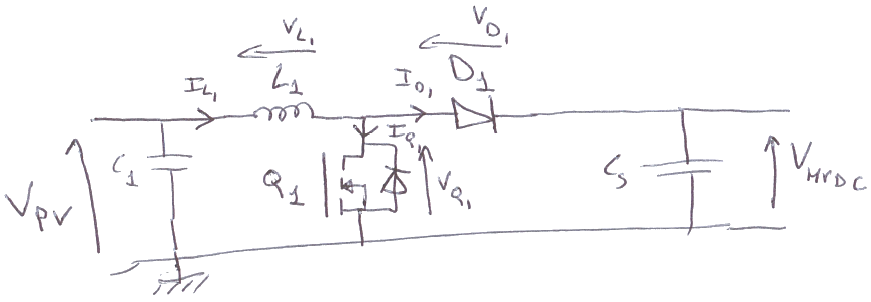
\includegraphics[width=\textwidth]{TD_Boost_2Q_Onduleur/fig/Boost.PNG}
\end{figure}

\begin{figure}[H]
    \centering
    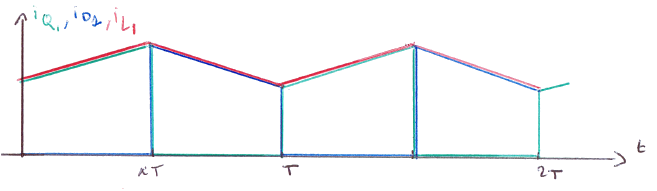
\includegraphics[width=\textwidth]{TD_Boost_2Q_Onduleur/fig/Boost_currents.PNG}
\end{figure}

\begin{figure}[H]
    \centering
    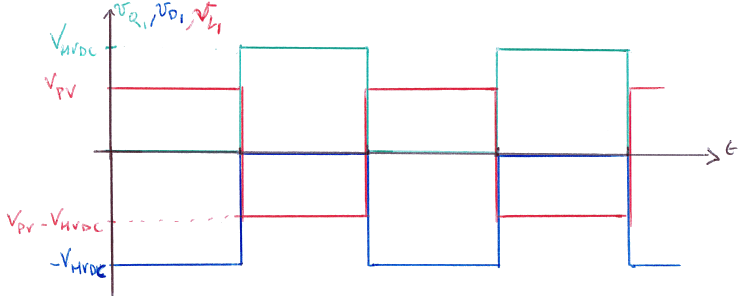
\includegraphics[width=\textwidth]{TD_Boost_2Q_Onduleur/fig/Boost_voltages.PNG}
\end{figure}
}

\ifthenelse{\equal{\Langue}{FR}}{
\item Déterminer l'expression de HVDC en fonction de la tension d'entrée, notée Vpv, et du rapport cyclique $\alpha$.
De même, exprimer la relation entre le courant Ipv (courant moyen dans L1) et le courant de sortie $I_{HVDC}$.
}{
\item Determine the expression of HVDC as a function of the input voltage, denoted Vpv, and the duty cycle $\alpha$. Similarly, express the relationship between the input current Ipv (average current in L1) and the output current $I_{HVDC}$.
}

\ifthenelse{\equal{\SuCorr}{CO}}{
$\begin{aligned}
    <v_{L1}> = 0 &\Rightarrow \alpha V_{PV} +(1-\alpha)(V_{PV} -V_{HVDC})=0\\
    &\Rightarrow V_{HVDC} = \dfrac{V_{PV}}{1-\alpha}
\end{aligned}$

\begin{itemize}
    \item \ifthenelse{\equal{\Langue}{FR}}{\underline{Pas de pertes}}{\underline{No losses}} $\Rightarrow V_{PV}\cdot I_{PV} = V_{HVDC} \cdot I_{HVDC}$
    
    $\Rightarrow I_{PV}= \dfrac{I_{HVDC}}{1-\alpha}$
\end{itemize}
}

\ifthenelse{\equal{\Langue}{FR}}{
\item Déterminer littéralement:
\item }{
\item Determine literally:
}

\begin{enumerate}

\ifthenelse{\equal{\Langue}{FR}}{
\item La tension maximale appliquée aux bornes de Q1 et D1.
\item Les valeurs moyennes et maximales des courants dans L1, Q1 et D1 en fonction de Ipv, $\Delta I$ et du rapport cyclique.
\item Résumer ces résultats dans un tableau de contraintes (utile pour le choix des composants).
}{
\item The maximum voltage applied to the terminals of Q1 and D1.
\item The average and maximum values of the currents in L1, Q1, and D1 as a function of Ipv, $\Delta I$, and the duty cycle.
\item Summarize these results in a constraints table (useful for component selection).
}

\ifthenelse{\equal{\SuCorr}{CO}}{
\begin{tabular}{|c|c|c|c|}
    \hline
    & Max Voltage & Max Current & Average Current \\
    \hline
    $L_1$ & $Max(V_{PV};|V_{PV}-V_{HVDC}|)$ & $I_{PV} + \dfrac{\Delta I}{2}$ & $I_{PV}$\\
    \hline
    $Q_1$ & $V_{HVDC}$ & $I_{PV} + \dfrac{\Delta I}{2}$ & $\alpha I_{PV}$ \\
    \hline
    $D_1$ & $V_{HVDC}$ & $I_{PV} + \dfrac{\Delta I}{2}$ & $(1-\alpha) I_{PV}$\\
    \hline
\end{tabular}
}

\end{enumerate}

\ifthenelse{\equal{\Langue}{FR}}{
On considère maintenant les deux BOOST en fonctionnement et se répartissant la puissance de façon égale. Les commandes de Q1 et Q2 sont synchrones.
Les conditions d'environnement sont les conditions STC ($1000 W/m^2$, $25^\circ C$).

On considère également une séquence de fonctionnement durant laquelle (1er cas extrême):
\begin{itemize}
\item la puissance consommée par la charge est maximale
\item la batterie n'est pas totalement chargée et consomme le différentiel de puissance entre la puissance consommée par la charge et la puissance fournie par les PV, qui correspond à la `` puissance crête'' totale.
\end{itemize}

\item Déterminer:
}{
Now, consider both BOOST converters operating and sharing the power equally. The environmental conditions are STC conditions ($1000 W/m^2$, $25^\circ C$).

We also consider an operating sequence in which (first extreme case):
\begin{itemize}
\item The power consumed by the load is maximum.
\item The battery is not fully charged and consumes the power difference between the power consumed by the load and the power supplied by the PV panels, which corresponds to the total ``peak'' power.
\end{itemize}

\item Determine:
}

\begin{enumerate}

\ifthenelse{\equal{\Langue}{FR}}{
\item La puissance totale $P_{cT}$ que peuvent fournir les PV compte tenu de l'irradiation.
}{
\item The total power $P_{cT}$ that the PV panels can provide considering the irradiation.
}

\ifthenelse{\equal{\SuCorr}{CO}}{
STC\@: 1 pannel: $250\ \text{W}_C$
$\Rightarrow 11$ \ifthenelse{\equal{\Langue}{FR}}{panneaux}{panels}:  $P_{TC} = 3000\ \text{W}_C$
}

\ifthenelse{\equal{\Langue}{FR}}{
\item La puissance qui transite dans chaque BOOST\@.
}{
\item The power flowing through each BOOST converter.
}

\ifthenelse{\equal{\SuCorr}{CO}}{
\ifthenelse{\equal{\Langue}{FR}}{A travers chaque BOOST}{Through each BOOST}\@: $\dfrac{3000}{2}=1500 \text {W}$
}

\ifthenelse{\equal{\Langue}{FR}}{
\item La puissance consommée par la batterie.
}{
\item The power consumed by the battery.
}

\ifthenelse{\equal{\SuCorr}{CO}}{
\ifthenelse{\equal{\Langue}{FR}}{Dans la batterie}{In the battery}: $3000 - \underbrace{1500 - 300}_{\text{\ifthenelse{\equal{\Langue}{FR}}{puissance max consommée}{max power consumed}}} = 1200 \text{ W}$
}

\end{enumerate}

\ifthenelse{\equal{\Langue}{FR}}{
\item Dans ces conditions de fonctionnement, pour chacun des deux BOOST déterminer:
}{
\item Under these operating conditions, for each of the two BOOST converters, determine:
}

\begin{enumerate}

\ifthenelse{\equal{\Langue}{FR}}{
\item La tension d'entrée Vpv.
}{
\item The input voltage Vpv.
}

\ifthenelse{\equal{\SuCorr}{CO}}{
1 \ifthenelse{\equal{\Langue}{FR}}{panneau}{panel} @ STC $\rightarrow V_{1PV} = 39 V$
$\Rightarrow 6$ \ifthenelse{\equal{\Langue}{FR}}{panneaux en série}{panels in series} $\rightarrow V_{PV} = 234 \text{ V}$
}

\ifthenelse{\equal{\Langue}{FR}}{
\item Le courant d'entrée Ipv.
}{
\item The input current Ipv.
}

\ifthenelse{\equal{\SuCorr}{CO}}{
1 Boost $\rightarrow P = 1500 \text{ W} \Rightarrow I_{PV} = \dfrac{1500}{234} = 6.4 \text{ A}$
}

\ifthenelse{\equal{\Langue}{FR}}{
\item Le rapport cyclique de commande des transistors.
}{
\item The control duty cycle of the transistors.
}

\ifthenelse{\equal{\SuCorr}{CO}}{
$V_{HVDC} = 500 \text{ V} \Rightarrow \alpha = \dfrac{V_{HVDC} - V_{PV}}{V_{HVDC}} = 0.53$
}

\ifthenelse{\equal{\Langue}{FR}}{
\item La valeur de L pour que $\Delta I$ représente 20 \% de Ipv.
}{
\item The value of L for which $\Delta I$ represents 20\% of Ipv.
}

\ifthenelse{\equal{\SuCorr}{CO}}{
$I_{PV} = 6.4 \text{ A} \Rightarrow \Delta I = 1.28 \text{ A}$ (20\% \ifthenelse{\equal{\Langue}{FR}}{de}{of} $I_{PV}$)
\newline \underline{$0 < t < \alpha T$}: $V_L = V_{PV} = L \dfrac{i_{PV}}{dt} \Rightarrow \Delta I = \dfrac{V_{PV}}{L}\alpha T$
\newline $\Rightarrow L = 1.93 \text{ mH}$
}

\ifthenelse{\equal{\Langue}{FR}}{
\item Les contraintes appliquées sur les composants de puissance Q et D (tension max., courant moyen et max.) 
}{
\item The constraints applied to the power components Q and D (maximum voltage, average and maximum current).
}

\ifthenelse{\equal{\SuCorr}{CO}}{
\begin{tabular}{|c|c|c|c|}
    \hline
    & \ifthenelse{\equal{\Langue}{FR}}{Tension max}{Max Voltage} & \ifthenelse{\equal{\Langue}{FR}}{Courant max}{Max Current} & \ifthenelse{\equal{\Langue}{FR}}{Courant moyen}{Average Current} \\
    \hline
    $Q_1$ & 500 V & 7 A & 3.4 A \\
    \hline
    $D_1$ & 500 V & 7.1 A & 3 A \\
    \hline
\end{tabular}
}

\end{enumerate}

\ifthenelse{\equal{\Langue}{FR}}{
On considère maintenant que la puissance consommée par la charge est la puissance minimale et que la batterie est totalement chargée (2nd cas extrême).

\item On suppose que les conditions sont toujours STC et que la tension de sortie d'un PV est de 44 V.
}{
Now, assume that the power consumed by the load is the minimum power and the battery is fully charged (second extreme case).

\item Suppose that the conditions are still STC conditions and that the output voltage of a PV panel is 44 V.
}

\begin{enumerate}

\ifthenelse{\equal{\Langue}{FR}}{
\item Déterminer la puissance fournie par chaque groupe de PV et le courant d'entrée de chaque BOOST\@.
}{
\item Determine the power supplied by each group of PV panels and the input current of each BOOST converter.
}

\ifthenelse{\equal{\SuCorr}{CO}}{
$V_{PV} = 6 \times 44 = 264 \text{ V}$
\vspace{0.25cm}

$\begin{array}{l l}
    \left\{\begin{array}{l l}
    \text{\ifthenelse{\equal{\Langue}{FR}}{Batterie chargée}{Battery charged}} &: P_{batt} = 0 \text{ W}\\
    \text{\ifthenelse{\equal{\Langue}{FR}}{charge min}{min load}} &: P_{load} = 300 \text{ W}
    \end{array}\right. \rightarrow \text{1 BOOST\@: } & P=150 \text{ W} \\
    & I_{PV} = \dfrac{150}{264} = 0.57 \text{ A}\end{array}$
}

\ifthenelse{\equal{\Langue}{FR}}{
\item Les BOOST fonctionnent-ils toujours en régime de conduction continue?
}{
\item Are the BOOST converters still operating in continuous conduction mode?
}

\ifthenelse{\equal{\SuCorr}{CO}}{
$I_{PV} < \dfrac{\Delta I}{2} \Rightarrow$ \underline{\ifthenelse{\equal{\Langue}{FR}}{Conduction discontinue}{Discontinuous mode}}
}

\ifthenelse{\equal{\Langue}{FR}}{
\item Représenter le courant d'entrée dans L ainsi que la tension à ses bornes.
}{
\item Represent the input current in L and the voltage across it.
}

\ifthenelse{\equal{\SuCorr}{CO}}{
\begin{figure}[H]
    \centering
    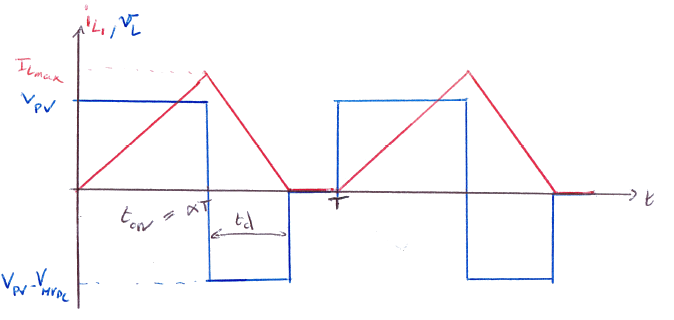
\includegraphics[width=\textwidth]{TD_Boost_2Q_Onduleur/fig/Boost_discontinuous.PNG}
\end{figure}
}

\ifthenelse{\equal{\Langue}{FR}}{
\item Exprimer le courant d'entrée Ipv en fonction de Vpv, HVDC, L, Fd et le temps de conduction du transistor $t_{on}$.
}{
\item Express the input current Ipv as a function of Vpv, HVDC, L, Fd, and the transistor conduction time $t_{on}$.
}

\ifthenelse{\equal{\SuCorr}{CO}}{
$<v_L> = 0 \Rightarrow V_{PV} \cdot I_{PV} = \dfrac{I_{Lmax}}{2}\cdot \dfrac{t_{on}+t_D}{T}$

\underline{$0 < t < \alpha T$}: $v_L = V_{PV} = L \dfrac{di_L}{dt} \Rightarrow I_{Lmax} = \dfrac{V_{PV}}{L} t_{on}$

$\Rightarrow I_{PV} = \dfrac{V_{PV}}{2 L}t_{on}\cdot F_d \cdot t_{on} \left(1+\dfrac{V_{PV}}{V_{HVDC}-V_{PV}}\right)$

$\Rightarrow I_{PV} = \dfrac{V_{PV} V_{HVDC}}{V_{HVDC}-V_{PV}}\cdot \dfrac{F_d}{2 L} \cdot t_{on}^2$
}

\ifthenelse{\equal{\Langue}{FR}}{
\item Déterminer la nouvelle valeur de rapport cyclique permettant de maintenir HVDC à 500 V.
}{
\item Determine the new value of the duty cycle to maintain HVDC at 500 V.
}

\ifthenelse{\equal{\SuCorr}{CO}}{
$t_{on} = 8.8 \mu \text{s} \rightarrow \alpha = 0.44$
}

\end{enumerate}
\end{enumerate}

\newpage
%%%%%%%% Partie 2 %%%%%%%
\ifthenelse{\equal{\Langue}{FR}}{
\section{Chargeur de Batterie (Half-Bridge)}

Pour permettre une alimentation en électricité durant la nuit, un pack de batteries est mis en place.

La structure de puissance associée aux batteries est celle d'un convertisseur réversible de type ``Half Bridge'' (Hacheur 2 quadrants). Ce convertisseur permet d'alimenter l'installation à partir du pack durant la nuit, et de recharger le pack à partir des PV pendant la journée.

\vspace{0.5cm}
Le schéma suivant présente cette structure:
}{
\section{Battery Charger (Half-Bridge)}

To provide electricity supply during the night, a battery pack is installed.

The power structure associated with the batteries is that of a reversible converter of the ``Half Bridge'' type (2-quadrant chopper). This converter allows powering the installation from the pack during the night and recharging the pack from the PV panels during the day.

\vspace{0.5cm}
The following diagram shows this structure:
}

\begin{figure}[ht]
\centering
\includegraphics[width=0.8\linewidth]{TD_Boost_2Q_Onduleur/fig/Archi_2Q.png}
\caption{2 Quadrant Chopper Architecture}
\end{figure}

\ifthenelse{\equal{\Langue}{FR}}{
Dans tous les cas, les boucles de régulation des BOOST et du Half-Bridge permettent de maintenir \textbf{HVDC = 500 V.}

La tension du pack batterie est supposée constante et égale à \textbf{Ubatt = 120 V} (38 éléments de 3.2 V / Technologie LiFePo4).

Une boucle de limitation du courant batterie incluse dans le BMS (Battery Management System) limite celui-ci à $I_{batt\_\max} = 10\ A$.

Les transistors Q3 et Q4 sont pilotés en commandes complémentaires à une fréquence fixe de 50 kHz. Les temps morts sont négligés.

Par la suite, le rapport cyclique désigne le rapport du temps de conduction de Q3 ramené à la période de découpage.
}{
In all cases, the control loops of the BOOST and Half-Bridge converters maintain \textbf{HVDC = 500 V.}

The battery pack voltage is assumed to be constant and equal to \textbf{Ubatt = 120 V} (38 elements of 3.2 V / LiFePo4 technology).

A battery current limiting loop included in the BMS (Battery Management System) limits it to $I_{batt\_\max} = 10\ A$.

Transistors Q3 and Q4 are driven in complementary control at a fixed frequency of 50 kHz. Dead times are neglected.

Hereafter, the duty cycle refers to the ratio of the conduction time of Q3 to the switching period.
}


\begin{enumerate}
\ifthenelse{\equal{\Langue}{FR}}{
\item Pour un rapport cyclique donné (0.3 par exemple) et en régime de conduction continue, représenter, pour des courants de charge ($I_{L3} > 0$) et de décharge de la batterie de mêmes valeurs absolues:
}{
\item For a given duty cycle (0.3 for example) and in continuous conduction mode, represent, for charge currents ($I_{L3} > 0$) and battery discharge currents of the same absolute values:
}

\begin{enumerate}
\ifthenelse{\equal{\Langue}{FR}}{
\item Les courants dans L3, Q3 et Q4.
}{
\item The currents in L3, Q3, and Q4.
}

\ifthenelse{\equal{\Langue}{FR}}{
\item La tension aux bornes de L3.
}{
\item The voltage across L3.
}

\ifthenelse{\equal{\Langue}{FR}}{
\item Présenter les sens de circulation du courant dans L3.
}{
\item Indicate the directions of current flow in L3.
}

\ifthenelse{\equal{\SuCorr}{CO}}{
\begin{figure}[H]
        \centering
        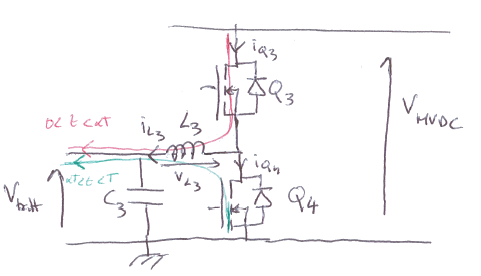
\includegraphics[width=0.9\textwidth]{TD_Boost_2Q_Onduleur/fig/HalfBridge.PNG}
    \end{figure}

    \begin{figure}[H]
        \centering
        \begin{minipage}[b]{0.45\textwidth}
            \centering \underline{Charge}
        \end{minipage}
        \hfill
        \begin{minipage}[b]{0.45\textwidth}
            \centering \underline{\ifthenelse{\equal{\Langue}{FR}}{Décharge}{Discharge}}
        \end{minipage}
        \vfill
        \begin{minipage}[b]{0.45\textwidth}
            \centering
            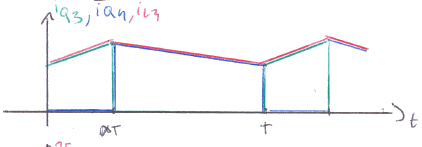
\includegraphics[width=\textwidth]{TD_Boost_2Q_Onduleur/fig/HalfBridge_current_charge.PNG}
        \end{minipage}
        \hfill
        \begin{minipage}[b]{0.45\textwidth}
            \centering
            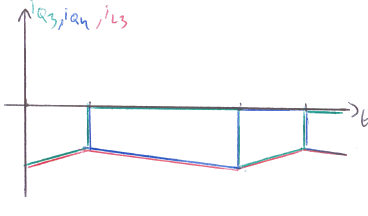
\includegraphics[width=\textwidth]{TD_Boost_2Q_Onduleur/fig/HalfBridge_current_discharge.PNG}
        \end{minipage}
        \vfill
        \begin{minipage}[b]{0.45\textwidth}
            \centering
            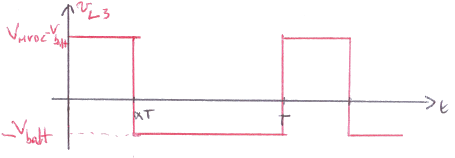
\includegraphics[width=\textwidth]{TD_Boost_2Q_Onduleur/fig/HalfBridge_voltage.PNG}
        \end{minipage}
        \hfill
        \begin{minipage}[b]{0.45\textwidth}
            \centering
            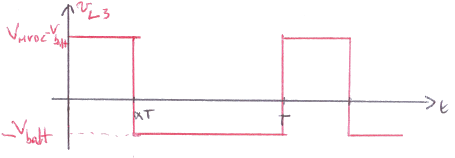
\includegraphics[width=\textwidth]{TD_Boost_2Q_Onduleur/fig/HalfBridge_voltage.PNG}
        \end{minipage}
    \end{figure}
}

\end{enumerate}


\ifthenelse{\equal{\Langue}{FR}}{
\item Exprimer la relation entre la tension batterie et HVDC en fonction du rapport cyclique de commande de Q3 noté $\alpha_{HB}$ (en régime de conduction continue).
}{
\item Express the relationship between the battery voltage and HVDC as a function of the control duty cycle of Q3 denoted $\alpha_{HB}$ (in continuous conduction mode).
}

\ifthenelse{\equal{\SuCorr}{CO}}{
$<v_L> = 0 \Rightarrow V_{batt} = \alpha_{HB} V_{HVDC}$
}


\ifthenelse{\equal{\Langue}{FR}}{
Dans un premier temps, on se place en journée pendant que le pack se recharge dans une configuration correspondante à la question 4 du TD\ \ref{sec:Convertisseur_BOOST}. Dans cette configuration, le courant de charge de la batterie est $I_{batt\_\max}$.

\item Le convertisseur Half Bridge fonctionne-t-il en ``Buck'' ou en ``Boost''? A quoi sert C3?
}{
Initially, we are in the daytime while the pack is being charged in a configuration corresponding to question 4 of TD\ \ref{sec:Convertisseur_BOOST}. In this configuration, the battery charging current is $I_{batt\_\max}$.

\item Is the Half-Bridge converter operating in ``Buck'' or ``Boost'' mode? What is the purpose of C3?
}

\ifthenelse{\equal{\SuCorr}{CO}}{
\begin{itemize}
    \item $P_{batt} = 1200 \text{ W} \rightarrow \text{\ifthenelse{\equal{\Langue}{FR}}{charge de la batterie}{battery charging}} \rightarrow \text{Half Bridge \ifthenelse{\equal{\Langue}{FR}}{en}{in} Buck}$
    \item $C_3$ \ifthenelse{\equal{\Langue}{FR}}{est utilisé pour filtrer les ondulations de courant hautes fréquences pour éviter qu'elles n'aillent dans la batterie}{is used to filter hight frequency current ripple so it does not flow in the Battery}
\end{itemize}
}

\ifthenelse{\equal{\Langue}{FR}}{
\item On souhaite que l'ondulation de courant dans L3 représente 30 \% de son courant moyen (soit 3 A). Déterminer:
}{
\item We want the ripple current in L3 to represent 30\% of its average current (i.e., 3 A). Determine:
}



\begin{enumerate}
\ifthenelse{\equal{\Langue}{FR}}{
\item Le rapport cyclique de commande de Q3.
}{
\item The control duty cycle of Q3.
}

\ifthenelse{\equal{\SuCorr}{CO}}{
$I_{batt} = \dfrac{P_{batt}}{V_{batt}}=\dfrac{1200}{120} = 10\text{ A} \rightarrow \Delta I = 3\text{ A}$

$V_{batt} = 120\text{ V}, V_{HVDC} = 500 \text{ V} \rightarrow \alpha_{HB} = 0.24$
}

\ifthenelse{\equal{\Langue}{FR}}{
\item La valeur à donner à L3
}{
\item The value to be given to L3.
}

\ifthenelse{\equal{\SuCorr}{CO}}{
\underline{$0 < t < \alpha T$}: $V_{L}= V_{HVDC} - V_{batt} = L \dfrac{di_L}{dt}$ 

$\Rightarrow \Delta I = \dfrac{V_{HVDC}-V_{batt}}{L} \alpha T \Rightarrow L = 600 \mu\text{H}$
}

\end{enumerate}



\ifthenelse{\equal{\Langue}{FR}}{
\item Pour ce point de fonctionnement, déterminer les contraintes en tension, courant maximum et courant moyen sur Q3 et Q4.
}{
\item For this operating point, determine the voltage, maximum current, and average current constraints on Q3 and Q4.
}

\ifthenelse{\equal{\SuCorr}{CO}}{
\begin{tabular}{|c|c|c|c|}
    \hline
    & Max Voltage & Max Current & Average Current \\
    \hline
    $Q_3$ & 500 V & 11.5 A & 2.4 A ($\alpha I_{batt}$) \\
    \hline
    $Q_4$ & 500 V & 11.5 A & 7.6 A ($(1-\alpha)I_{batt}$)\\
    \hline
    \multicolumn{2}{c}{} &  \multicolumn{1}{c}{($I_{bat} + \dfrac{\Delta I}{2}$)} & \multicolumn{1}{c}{}
\end{tabular}
}


\ifthenelse{\equal{\Langue}{FR}}{
On se place toujours durant la journée, mais maintenant dans une configuration où l'installation appelle sa puissance maximale (1800 W). Les conditions météorologiques sont telles que les PV ne peuvent fournir que 1000 W (rendement des Boost compris).

\item Quelle est la puissance fournie par la batterie et que vaut son courant?
}{
We are still in the daytime, but now in a configuration where the installation calls for its maximum power (1800 W). The weather conditions are such that the PV panels can only provide 1000 W (including Boost efficiencies).

\item What is the power supplied by the battery and what is its current?
}

\ifthenelse{\equal{\SuCorr}{CO}}{
$\left\{\begin{array}{l}P_{load} = 1800 \text{ W}\\ P_{PV}=1000\text{ W}\end{array}\right. \rightarrow \left\{\begin{array}{l}P_{batt}=-800 \text{ W}\\
I_{batt} = -6.7\text{ A}\end{array}\right.$
}

\ifthenelse{\equal{\Langue}{FR}}{
\item Le fonctionnement du HB est-il ``Buck'' ou ``Boost''?
}{
\item Is the Half-Bridge operation ``Buck'' or ``Boost''?
}

\ifthenelse{\equal{\SuCorr}{CO}}{
\ifthenelse{\equal{\Langue}{FR}}{
Half Bridge en fonctionnement Boost $\rightarrow$ énergie fournie par la batterie
}{Half Bridge in Boost operation $\rightarrow$ energy supplied by the Battery
}}

\ifthenelse{\equal{\Langue}{FR}}{
\item Que vaut le rapport cyclique de commande de Q3?  Le convertisseur HB fonctionne-t-il toujours en régime de conduction continue? Représenter les courants dans L3, Q3 et Q4 et la tension $V_{L3}$ en précisant les valeurs numériques remarquables. Donner les schémas équivalents aux deux phases de fonctionnement en précisant les sens de circulation des courants.
}{
\item What is the control duty cycle of Q3? Is the HB converter still operating in continuous conduction mode? Represent the currents in L3, Q3, and Q4 and the voltage $V_{L3}$ indicating the remarkable numerical values. Provide the equivalent diagrams for the two operating phases indicating the directions of current flow.
}

\ifthenelse{\equal{\SuCorr}{CO}}{
$\alpha_{HB}=0.24$ ($V_{HVDC}$ \ifthenelse{\equal{\Langue}{FR}}{et}{and} $V_{bat}$ \ifthenelse{\equal{\Langue}{FR}}{n'ont pas changé}{are still the same})
    
\ifthenelse{\equal{\Langue}{FR}}{Pas de conduction discontinue dans un half bridge (réversibilité en courant)}{No discontinuous mode for Half Bridge (current reversible)}

$\rightarrow$ \ifthenelse{\equal{\Langue}{FR}}{le courant dans $L_3$ est simplement négatif}{current in $L_3$ is just negative}

\begin{center}
    \begin{minipage}[c]{0.2\textwidth}
        \centering
        \underline{$0 < t < \alpha_{HB} T$}:
    \end{minipage}
    \hfill
    \begin{minipage}[c]{0.45\textwidth}
        \centering
        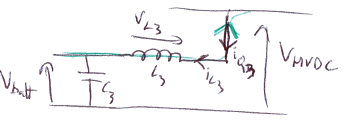
\includegraphics[width=\textwidth]{TD_Boost_2Q_Onduleur/fig/HalfBridge_1.PNG}
    \end{minipage}
    \hfill
    \begin{minipage}[c]{0.25\textwidth}
        \centering
        $V_{L_3}=V_{HVDC} - V_{batt}$
    \end{minipage}
    %\vfill
    \begin{minipage}[c]{0.2\textwidth}
        \centering
        \underline{$\alpha_{HB} T < t < T$}:
    \end{minipage}
    \hfill
    \begin{minipage}[c]{0.5\textwidth}
        \centering
        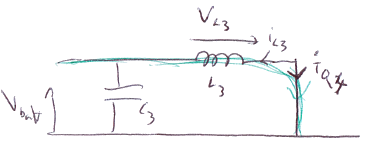
\includegraphics[width=\textwidth]{TD_Boost_2Q_Onduleur/fig/HalfBridge_2.PNG}
    \end{minipage}
    \hfill
    \begin{minipage}[c]{0.2\textwidth}
        \centering
        $V_{L_3}=- V_{batt}$
    \end{minipage}
\end{center}

\begin{figure}[H]
    \centering
    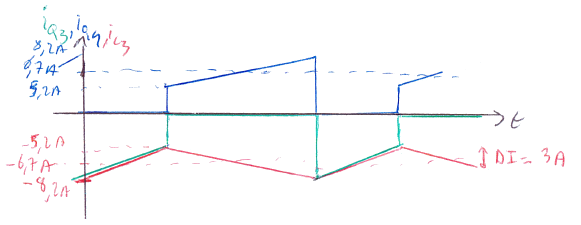
\includegraphics[width=\textwidth]{TD_Boost_2Q_Onduleur/fig/HalfBridge_current.PNG}
\end{figure}
}

\ifthenelse{\equal{\Langue}{FR}}{
\item La nuit, la batterie fournie seule l'énergie à l'installation et la puissance consommée est de 300 W. On suppose que le rendement du HB est unitaire.
}{
\item During the night, the battery alone supplies power to the installation and the power consumed is 300 W. We assume that the HB efficiency is unity.
}


\begin{enumerate}

\ifthenelse{\equal{\Langue}{FR}}{
\item Déterminer la valeur du rapport cyclique de Q3 pour maintenir HVDC à 500 V
}{
\item Determine the value of the control duty cycle of Q3 to maintain HVDC at \hbox{500 V}.
}

\ifthenelse{\equal{\SuCorr}{CO}}{
$P = 300 \text{ W} \rightarrow I_{batt} = -2.8 \text{ A}$
}

\ifthenelse{\equal{\Langue}{FR}}{
\item Représenter le courant dans L3 en précisant sa valeur moyenne.
}{
\item Represent the current in L3 indicating its average value.
}

\ifthenelse{\equal{\SuCorr}{CO}}{
$\alpha_{HB} = 0.24$ \ifthenelse{\equal{\Langue}{FR}}{(Même valeurs de $V_{batt}$ et $V_{HVDC}$)}{(Still same values of $V_{batt}$ and $V_{HVDC}$)}

\begin{figure}[H]
    \centering
    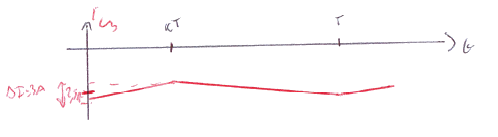
\includegraphics[width=\textwidth]{TD_Boost_2Q_Onduleur/fig/HalfBridge_currentC3.PNG}
\end{figure}
}

\end{enumerate}


\ifthenelse{\equal{\Langue}{FR}}{
\item En tenant compte d'un rendement global du [HB + Onduleur] de 90 \%, quelle doit être la capacité minimale (en Ah) du pack pour maintenir une autonomie durant 16h00 d'affilée et avec un taux de décharge maximum de 90 \% (sur cette période, les phases à puissance maximale n'apparaissent pas).
}{
\item Taking into account a global efficiency of [HB + Inverter] of 90\%, what should be the minimum capacity (in Ah) of the pack to maintain autonomy for 16 consecutive hours with a maximum discharge rate of 90\% (during this period, the phases at maximum power do not occur).
}

\ifthenelse{\equal{\SuCorr}{CO}}{
$P=300 \text{ W}$ \hspace{1cm} $\eta = 90\% \Rightarrow P_{batt} = 333 \text{ W}$

\ifthenelse{\equal{\Langue}{FR}}{Pour}{For} 16h $\rightarrow E_{batt} = 5.3 \text{ kWh}$

\ifthenelse{\equal{\Langue}{FR}}{Profondeur de décharge max}{Max discharge} 90\% $\rightarrow E_{batt TOTAL} = \dfrac{E_{batt}}{0.9} = 5.9 \text{ kWh}$

$V_{batt} = 120 \text{ V} \Rightarrow C_{batt} = 50 \text{ Ah}$
}

\end{enumerate}

\newpage
%%%%%%%% Partie 3 %%%%%%%
\ifthenelse{\equal{\Langue}{FR}}{
\section{Onduleur monophasé MLI sur charge RL}
}{
\section{Single-phase PWM Inverter on RL Load}
}

\ifthenelse{\equal{\Langue}{FR}}{
On s'intéresse maintenant à l'onduleur monophasé. Le réseau est modélisé par une charge R-L série. Le schéma de principe est le suivant:
}{
Now we focus on the single-phase inverter. The grid is modeled by a series R-L load. The block diagram is as follows:
}

\begin{figure}[ht]
\centering
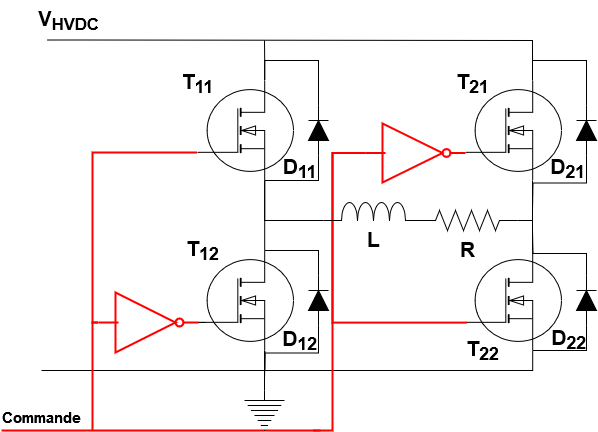
\includegraphics[width=0.8\linewidth]{TD_Boost_2Q_Onduleur/fig/Onduleur.png}
\end{figure}


\begin{itemize}
\setlength\itemsep{-1mm}
\ifthenelse{\equal{\Langue}{FR}}{
\item Les transistors fonctionnent en MLI à une fréquence de découpage $F_d$ très grande devant la fréquence de la tension à reconstituer en sortie.
\item Le rapport cyclique est variable dans le temps et sera noté: $\alpha(t) = 0.5 + \delta_\alpha \sin(\omega .t)$.
}{
\item The transistors operate in PWM at a switching frequency $F_d$ much higher than the frequency of the output voltage to be reconstructed.
\item The duty cycle varies over time and will be denoted as $\alpha(t) = 0.5 + \delta_\alpha \sin(\omega t)$.
}
\end{itemize}

\ifthenelse{\equal{\Langue}{FR}}{
Par la suite, on désigne par:
}{
Hereafter, we refer to:
}

\begin{itemize}
\setlength\itemsep{-1mm}
\ifthenelse{\equal{\Langue}{FR}}{
\item $V_0$: la tension aux bornes de l'ensemble $L - R$ (tension de sortie de l'onduleur).
\item $I_R$: le courant dans la charge $R - L$
}{
\item $V_0$: the voltage across the $L - R$ combination (inverter output voltage).
\item $I_R$: the current in the R-L load.
}
\end{itemize}

\ifthenelse{\equal{\Langue}{FR}}{
Les principales caractéristiques de la charge sont:
}{
The main characteristics of the load are:
}

\begin{itemize}
\setlength\itemsep{-1mm}
\ifthenelse{\equal{\Langue}{FR}}{
\item Schéma équivalent: $R - L$ série, avec $L = 30 mH$
\item Puissance nominale: 1500 W
\item Tension nominale aux bornes de $R$: $U_{Rn} = 230 V$ (valeur efficace)
%\item Après la mise sous tension, la puissance absorbée par la charge évolue linéairement de 300 à 500 W pendant 300 secondes, puis se stabilise à 500 W.
%\item Dans le même intervalle de temps, la tension efficace aux bornes de $R$ (notée : $U_R$), évolue linéairement de 40 à 100 V.
}{
\item Equivalent circuit: series $R - L$, with $L = 30 mH$
\item Rated power: 1500 W
\item Rated voltage across $R$: $U_{Rn} = 230 V$ (rms value)
%\item After startup, the power absorbed by the load increases linearly from 300 to 500 W over 300 seconds, then stabilizes at 500 W.
%\item In the same time interval, the rms voltage across $R$ (denoted: $U_R$) increases linearly from 40 to 100 V.
}
\end{itemize}

\begin{enumerate}
\ifthenelse{\equal{\Langue}{FR}}{
%\item Sur un même graphe, et durant les 400 secondes suivant la mise sous tension, représenter les évolutions :
%
%\begin{enumerate}
%\item de la puissance absorbée par la charge
%\item de la tension aux bornes de $R$ : $U_R$
%\item du courant efficace dans la charge $I_R$
%\end{enumerate}

\item Tension de sortie $V_0$
}{
%\item On the same graph, and during the 400 seconds following startup, represent the evolutions of:
%
%\begin{enumerate}
%\item the power absorbed by the load
%\item the voltage across $R$: $U_R$
%\item the rms current in the load $I_R$
%\end{enumerate}

\item Output voltage $V_0$
}

\begin{enumerate}
\ifthenelse{\equal{\Langue}{FR}}{
\item Représenter l'allure de la tension de sortie pour un rapport cyclique $\alpha > 0.5$ et sur une période de découpage
}{
\item Represent the shape of the output voltage for a duty cycle $\alpha > 0.5$ over one switching period.
}

\ifthenelse{\equal{\SuCorr}{CO}}{
\begin{figure}[H]
    \centering
    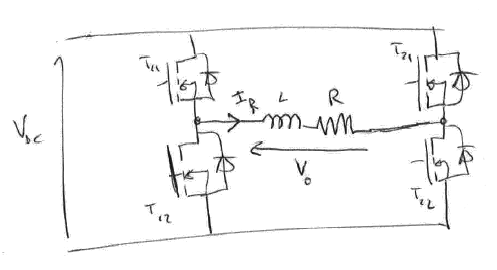
\includegraphics[width=\textwidth]{TD_Boost_2Q_Onduleur/fig/Inverter.PNG}
\end{figure}

\[\alpha(t) = 0.5 + \delta_\alpha \sin(\omega t)\]

\begin{figure}[H]
    \centering
    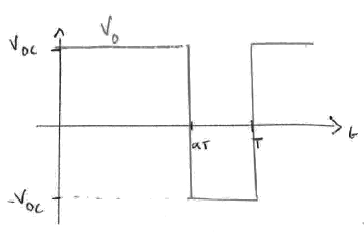
\includegraphics[width=\textwidth]{TD_Boost_2Q_Onduleur/fig/Inverter_voltage.PNG}
\end{figure}
}


\ifthenelse{\equal{\Langue}{FR}}{
\item Exprimer la valeur moyenne de $V_o$ sur une période de découpage en fonction du rapport cyclique $\alpha$ et de $V_{DC}$
}{
\item Express the average value of $V_o$ over one switching period as a function of the duty cycle $\alpha$ and $V_{DC}$.
}

\ifthenelse{\equal{\SuCorr}{CO}}{
$<V_0> = (2\alpha - 1) V_{DC}$
}

\ifthenelse{\equal{\Langue}{FR}}{
\item Exprimer l'évolution temporelle de la valeur moyenne (sur une période de découpage) de la tension de sortie \hbox{$<V_0>(t)$} en fonction de $V_{DC}$ et $\delta_\alpha$
}{
\item Express the time-varying average value (over one switching period) of the output voltage $<V_0>(t)$ as a function of $V_{DC}$ and $\delta_\alpha$.
}

\ifthenelse{\equal{\SuCorr}{CO}}{
$<V_0> (t) = (2\alpha(t) - 1 ) V_{DC} = 2\delta_\alpha V_{DC} \sin(\omega t)$
}

\ifthenelse{\equal{\Langue}{FR}}{
\item Déterminer la valeur efficace de $<V_0>(t)$ (notée $V_{0\ eff}$) en fonction de $V_{HVDC}$ et $\delta_\alpha$
}{
\item Determine the rms value of $<V_0>(t)$ (denoted $V_{0\ eff}$) as a function of $V_{HVDC}$ and $\delta_\alpha$.
}

\ifthenelse{\equal{\SuCorr}{CO}}{
$V_{0 eff} = \sqrt{2} \delta_\alpha V_{DC}$
}

\ifthenelse{\equal{\Langue}{FR}}{
\item En négligeant la composante de courant due au découpage, donner l'expression du courant dans $R$ ($I_R(t)$) en prenant $<V_0>(t)$ en référence de phase
}{
\item Neglecting the current component due to switching, give the expression of the current in $R$ ($I_R(t)$) taking $<V_0>(t)$ as the reference phase.
}

\ifthenelse{\equal{\SuCorr}{CO}}{

}

\ifthenelse{\equal{\Langue}{FR}}{
\item Exprimer la valeur efficace du courant dans $R$ en fonction de $V_{0\ eff}$, $R$, $L$ et $\omega$
}{
\item Express the rms value of the current in $R$ as a function of $V_{0\ eff}$, $R$, $L$, and $\omega$.
}

\ifthenelse{\equal{\SuCorr}{CO}}{
$I_{R eff} = \dfrac{V_{0 eff}}{\sqrt{R^2 + {(L\omega)}^2}}$
}

\ifthenelse{\equal{\Langue}{FR}}{
\item Exprimer le déphasage $\varphi$ entre $I_R(t)$ et $<V_0>(t)$ en fonction de $R$, $L$ et $\omega$
}{
\item Express the phase shift $\varphi$ between $I_R(t)$ and $<V_0>(t)$ as a function of $R$, $L$, and $\omega$.
}

\ifthenelse{\equal{\SuCorr}{CO}}{
$\tan \delta = \dfrac{L\omega}{R}\Rightarrow \varphi = \arctan(\dfrac{L\omega}{R})$
}

\ifthenelse{\equal{\Langue}{FR}}{
\item Exprimer le facteur de puissance de la charge $RL$ en fonction de $R$, $L$ et $\omega$
}{
\item Express the power factor of the RL load as a function of $R$, $L$, and $\omega$.
}

\ifthenelse{\equal{\SuCorr}{CO}}{
$pf=\cos\varphi=\cos(\arctan(\dfrac{L\omega}{R}))$
}

\ifthenelse{\equal{\Langue}{FR}}{
\item Exprimer la puissance dans $R$ en fonction de $\delta_\alpha$, $V_{HVDC}$, $R$, et $\varphi$.
}{
\item Express the power in $R$ as a function of $\delta_\alpha$, $V_{HVDC}$, $R$, and $\varphi$.
}

\ifthenelse{\equal{\SuCorr}{CO}}{
$\begin{aligned}P_R &=R \cdot I_{R eff}^2= \dfrac{R V_{0 eff}^2}{R^2 + {8(L\omega)}^2}= \dfrac{2 R \delta_\alpha^2 V_{DC}^2}{R^2 + {(L\omega)}^2}\\
    &= \dfrac{2\delta_\alpha^2 V_{DC}^2}{R} \cdot \dfrac{1}{1+ \tan^2 \varphi} 
\end{aligned}$
}

\end{enumerate}

\ifthenelse{\equal{\Langue}{FR}}{
\item Fonctionnement à puissance nominale (1500W).

Pour rappel, la tension d'alimentation $V_{HVDC}$ est la tension du bus continu, $V_{HVDC}=500 V$. La fréquence de la tension reconstituée ($<V_0>(t)$) est de \textbf{50 Hz}.
}{
\item Operation at rated power (1500W).

As a reminder, the supply voltage $V_{HVDC}$ is the DC bus voltage, $V_{HVDC}=500 V$. The frequency of the reconstructed voltage ($<V_0>(t)$) is \textbf{50 Hz}.
}

\begin{enumerate}
\ifthenelse{\equal{\Langue}{FR}}{
\item Déterminer la valeur de $R$ pour ce point de fonctionnement
}{
\item Determine the value of $R$ for this operating point.
}

\ifthenelse{\equal{\SuCorr}{CO}}{
$P_R=1500 \text{ W} \hspace{1cm} U_{Rn} = 230 \text{ V} \Rightarrow I_{Rn} = \dfrac{P_R}{U_{Rn}} = 6.5 \text{ A}$

$P_R = R \cdot I_{Rn}^2 \Rightarrow R = \dfrac{P_R}{I_{Rn}^2} = 35.3 \Omega$

\ifthenelse{\equal{\Langue}{FR}}{Ou}{Or} $P_R = 500 \text{ W} = \dfrac{U_{Rn}^2}{R} \Rightarrow R \dfrac{U_{Rn}^2}{P_R} = \dfrac{230^2}{1500} = 35.3 \Omega$
}

\ifthenelse{\equal{\Langue}{FR}}{
\item Déterminer la valeur du facteur de puissance
}{
\item Determine the power factor value.
}

\ifthenelse{\equal{\SuCorr}{CO}}{
$L=30 \text{ mH} \hspace{1cm} f=50 \text{ Hz} \Rightarrow \varphi = \arctan(\dfrac{L\omega}{R}) = 0.26 \text{ rad }(15^\circ)$

$\cos \varphi = 0.97$
}

\ifthenelse{\equal{\Langue}{FR}}{
\item Etablir le diagramme de Fresnel liant $V_0$, $I_R$ et $U_R$
}{
\item Establish the Fresnel diagram relating $V_0$, $I_R$, and $U_R$.
}

\ifthenelse{\equal{\SuCorr}{CO}}{
\begin{figure}[H]
    \centering
    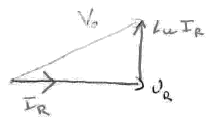
\includegraphics[width=0.5\textwidth]{TD_Boost_2Q_Onduleur/fig/Inverter_Fresnel.PNG}
\end{figure}
}

\ifthenelse{\equal{\Langue}{FR}}{
\item Déterminer la valeur de la tension aux bornes de $L$
}{
\item Determine the value of the voltage across $L$.
}

\ifthenelse{\equal{\SuCorr}{CO}}{
$I_R= 6.5 \text{ A} \rightarrow V_L = L \omega I_R = 61.23 \text{ V}$
}

\ifthenelse{\equal{\Langue}{FR}}{
\item Déterminer la valeur à donner à $V_{0\ eff}$
}{
\item Determine the value to be given to $V_{0\ eff}$.
}

\ifthenelse{\equal{\SuCorr}{CO}}{
$V_{0 eff} = \sqrt{U_R^2 + V_L^2} = 238 \text{ V}$
}

\ifthenelse{\equal{\Langue}{FR}}{
\item Déterminer la valeur à donner à $\delta_\alpha$ pour obtenir ce point de fonctionnement
}{
\item Determine the value to be given to $\delta_\alpha$ to achieve this operating point.
}

\ifthenelse{\equal{\SuCorr}{CO}}{
$V_{0 eff} = \sqrt{2} \delta_\alpha V_{DC}$ \ifthenelse{\equal{\Langue}{FR}}{avec}{with} $V_{DC} = 500 \text{ V} \Rightarrow \delta_\alpha = \dfrac{V_{0 eff}}{\sqrt{2} V_{DC}} = 0.34$
}

%\ifthenelse{\equal{\Langue}{FR}}{
%\item Déterminer les variations possibles de $\delta_\alpha$ compte tenu des variations possibles de la valeur efficace de la tension réseau (pour maintenir le point de fonctionnement nominal)
%\item En gardant la valeur de $R$, déterminer la puissance maximale transférable dans $R$ pour une tension réseau de 230 V efficace
%}{
%\item Determine the possible variations of $\delta_\alpha$ considering the possible variations of the rms value of the grid voltage (to maintain the nominal operating point).
%\item Keeping the value of $R$, determine the maximum power transferable to $R$ for a grid voltage of 230 V rms.
%}
\end{enumerate}

%\ifthenelse{\equal{\Langue}{FR}}{
%\item Lors du démarrage (à la mise sous tension) quand la tension réseau est à son nominal (230 V), déterminer :
%
%\begin{enumerate}
%\item le facteur de puissance
%\item la valeur à donner à $V_0$ (valeur efficace)
%\item l'expression du rapport cyclique
%\end{enumerate}
%}{
%\item During startup (at power-up) when the grid voltage is at its nominal value (230 V), determine:
%
%\begin{enumerate}
%\item the power factor
%\item the value to be given to $V_0$ (rms value)
%\item the expression of the duty cycle
%\end{enumerate}
%}

\ifthenelse{\equal{\Langue}{FR}}{
\item Déterminer la tension maximale à l'état bloqué et le courant maximum pour chaque interrupteur de l'onduleur (la composante de courant à la fréquence de découpage est toujours négligée)
}{
\item Determine the maximum voltage in the blocked state and the maximum current for each inverter switch (the current component at the switching frequency is always neglected).
}

\ifthenelse{\equal{\SuCorr}{CO}}{
\ifthenelse{\equal{\Langue}{FR}}{Tension max}{Max voltage}: $\dfrac{V_{DC}}{2} = 250 \text{ V}$

\ifthenelse{\equal{\Langue}{FR}}{Courant max}{Max current}: $\dfrac{V_{0 eff} \sqrt{2}}{\sqrt{R^2 + {(L\omega)}^2}} = \dfrac{\sqrt{2} \delta_\alpha V_{DC} \sqrt{2}}{\sqrt{R^2 + {(L\omega)}^2}} = 9.3 \text{ A}$
}

\end{enumerate}